\section{\textsc{Ei im Näpfchen}}

\subsection*{Zutaten für 2 Schälchen:}

\begin{tabular}{p{7.5cm} p{7.5cm}}
	& \\
	2 Eier & Butter zum Einfetten \\
	Salz \& Pfeffer &
\end{tabular}

\subsection*{Serviervorschlag:}

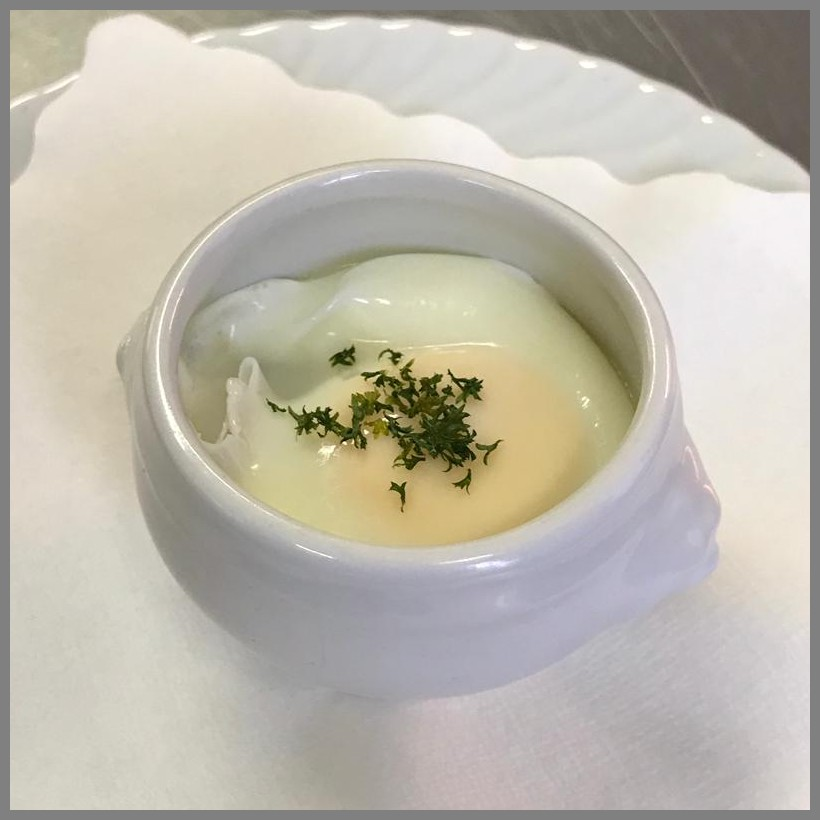
\includegraphics[width=\textwidth]{img/ei_naepfchen.jpg} \cite{eiimnaepfchen}

\subsection*{So geht's:}

\begin{tabular}{p{15cm}}
	\\
  Die Förmchen mit Butter einfetten.\\
  Jeweils ein Ei pro Person in jeweils ein Näpfchen aufschlagen. \\
  Mit Salz und Pfeffer würzen.\\
  Einen Topf zu 1/3 mit Wasser füllen. Langsam zum Kochen bringen.\\
  Die Näpfchen in das leicht kochende Wasser stellen.\\
  Deckel auf den Topf und das Ganze etwa 20min garen lassen.\\
  Vorsichtig aus dem Topf heben und servieren.\\
  %\vspace{0.5cm}
  \textbf{Tipp:} Das Gericht kann je nach Geschmack variiert werden. Es können noch Zutaten wie, Käse, Speck oder Zwiebeln hinzugefügt werden. Ebenso kann mit den Gewürzen „gespielt“ werden. Frische Kräuter passen perfekt dazu.
\end{tabular}
